\documentclass{article}
% Author: Luan Leal
% Last update: 2024-12-03

% ----------------------------

% ----------------------------   IMPORTS   ----------------------------
\usepackage{amssymb, amsthm, amsmath, geometry, siunitx, caption, float, graphicx}
\usepackage{enumitem}
\usepackage[utf8]{inputenc}
\usepackage[onehalfspacing]{setspaceenhanced}
\usepackage[brazil]{babel} % Adaptação ao pt-br
\usepackage{hyperref} % Usado para inserir links
\usepackage[capitalize, brazilian, noabbrev]{cleveref} % Referência adaptada ao pt-br
\usepackage{subcaption}
\usepackage{makecell}
\usepackage[num,overcite]{abntex2cite}

% ----------------------------   LAYOUT   ----------------------------
\citebrackets[]
\geometry{a4paper, lmargin=3cm, tmargin=3cm, rmargin=2cm, bmargin=2cm}
\onehalfspacing
%\setlength{\parindent}{45pt}
\sisetup{output-decimal-marker = {,}}

% ----------------------------  THEOREMS  ----------------------------
% -Ambiente de definição
\theoremstyle{definition}
\newtheorem{dfn}{Definição}[section]

% -Ambiente de observação
\theoremstyle{remark}
\newtheorem{obs}{Observação}

% -Ambiente de lema
\theoremstyle{definition}
\newtheorem{lema}{Lema}

% -Ambiente de exemplo
\theoremstyle{definition}
\newtheorem{xp}{Exemplo}[section]

% -Ambiente de proposição
\newtheorem{prop}{Proposição}

% -Ambiente de teorema e demonstração
\theoremstyle{plain}
\newtheorem{thm}{Teorema}
\theoremstyle{remark}
\newtheorem*{dms}{Demonstração}

% -Ambiente de exercício e resolução
\theoremstyle{definition}
\newtheorem{xcs}{Exercício}
\theoremstyle{remark}
\newtheorem*{rsl}{Resolução}

% ----------------------------  COMMANDS  ----------------------------
%\newcommand{\RR}{\mathbb{R}} % \mathbb{R} = \RR
%\newcommand{\ZZ}{\mathbb{Z}} % \mathbb{Z} = \ZZ

\author{Luan Leal (15470820);
; Matheus Queiroz (15479562);\\ Micael Baruch (15578823)}
\title{Relatório 2 --- Determinação do equilíbrio químico} 

\captionsetup{margin=10pt,font=small,labelfont=bf,labelsep=period}

\begin{document}
\maketitle

\section{Equilíbrios envolvidos no experimento}

De maneira simplificada, a reação cujo equilíbrio estamos interessados em acompanhar é a seguinte:
\begin{align*}
    \ce{Fe^{3+}_{aq} + SCN^-_{aq} <-->[{K_1}][{K_2}] {[Fe(SCN)]}^{2+}_{aq}}
\end{align*}

Em que \(K_1 = \cfrac{[{[Fe(SCN)]}^{2+}]}{[Fe^{3+}][SCN^-]} \) e \(K_2 = \cfrac{1}{K_1}\).

No entanto, estamos adicionando \ce{Fe(NO3)3} como fonte de íons ferro e \ce{KSCN} como fonte de íons tiocianato. Neste caso, o real equilíbrio é dado por:

\begin{align*}
    \ce{Fe(NO3)3 + KSCN ->[{K_3}] Fe^{3+}_{aq} + 3NO3^-_{aq} + SCN^-_{aq} + K^+_{aq} <-->[{K_1}][{K_2}] {[Fe(SCN)]}^{2+}_{aq} + 3NO3^-_{aq} + K^+_{aq}}
\end{align*}

Simultaneamente, pode ocorrer reação entre os íons férricos e a água:

\begin{align*}
    \ce{Fe^{3+}_{aq} + 2H2O_l <-->[{K_4}][{K_5}] {(Fe(OH))}^{2+}_{aq} + H3O^+_{aq}}
\end{align*}

Ainda assim, como os sais são extremamente solúveis, pode-se considerar que toda quantidade colocado torna-se íon. Quanto à reação com íons férricos e água, para isto a solução de ácido nítrico \qty{0,1}{M} é adicionada em lugar de água pura. Isto porque o ácido nítrico é um ácido forte, formando íons \ce{H3O^+} com a água, isto faz com que o equilíbrio da reação de ferro com água tenda para formação de íons ferro livres.


\section{Determinando a curva de calibração do \ce{{[Fe(SCN)]}^{2+}}}
Para determinação da curva de calibração foram feitas soluções ricas em \ce{FeNO3} em comparação ao \ce{KSCN}. O objetivo disto é que desta forma há excesso de íons férricos de tal forma que toda concentração disponível de \ce{KSCN} reage para formar \ce{Fe(SCN)}. Ou seja, a concentração final de \ce{Fe(SCN)} é igual à concentração inicial de \ce{KSCN}. Tirando a média dos dados dos diferentes grupos da sala obtivemos a curva de calibração descrita na \cref{curvaPadrao}

\begin{figure}[H]
    \centering
    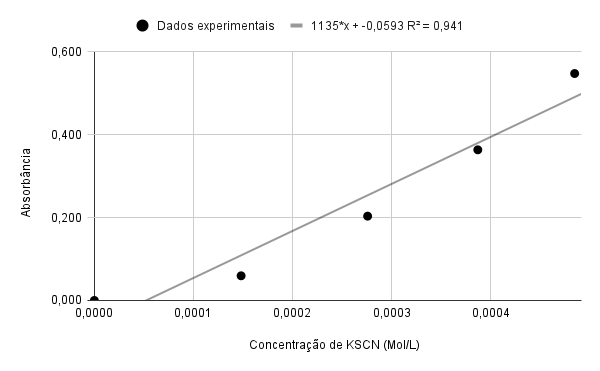
\includegraphics[width=.5\linewidth]{fig/curvaPadrao}
    \caption{Curva de calibração do \ce{Fe(SCN)} obtida pela média dos valores experimentais dos grupos da sala. A equação de reta que descreve a curva está apresentada na parte superior da figura.}\label{curvaPadrao}
\end{figure}

\section{Determinando a constante de formação do \ce{{[Fe(SCN)]}^{2+}}}

Para determinar a constante de formação do \ce{{[Fe(SCN)]}^{2+}} foi necessário extrair dos dados de absorbância obtidos qual era a concentração de \ce{{[Fe(SCN)]}^{2+}}. Para tanto, utilizamos a equação de reta obtida por regressão linear considerando o intercepto como zero: \(A = 976 c\), onde \(A\) é a absorbância e \(c\) é a concentração de \ce{{[Fe(SCN)]}^{2+}}. Os valores de concentração e da constante de formação \(K_1\) obtidos para cada concentração inicial de \ce{KSCN} estão resumidos na \cref{concFeSCN}.

\begin{table}[h]
    \centering
    \begin{tabular}{c c c}
        \hline
        \ce{[KSCN]}/(M x 1000) & \ce{[{[Fe(SCN)]}^{2+}]}/(M x 1000) & K_1/ (\(\frac{1}{M}\) x 1000) \\
        \hline
        0,2 & 0,157 & 4,3\\
        0,4 & 0,320 & 5,9\\
        0,6 & 0,477 & 7,4\\
        0,8 & 0,642 & 11,4\\
        --- & Média: & 7,3\\
        \hline
    \end{tabular}
    \caption{Valores de concentração de \ce{[{[Fe(SCN)]}^{2+}]} e de constante de formação obtidos pela absorbância para cada valor inicial de \ce{[KSCN]}}\label{concFeSCN}
\end{table}

Os valores obtidos na literatura são de \qty{179}{\liter\per\mol}. Isto difere do valor calculado por \qty{178,99}{\liter\per\mol}, ou seja, uma diferença de \(99,99\%\). Algum desvio seria esperado devido à erros de execução, embora compensados pelas replicatas entre diferentes grupos. Também seria possível que houvesse erro devido à variações de temperatura, visto que a temperatura também afeta o equilíbrio. Porém, em vista da temperatura ter se mantido relativamente constante e próxima de \qty{25}{\celsius} isto também não justifica a diferença observada. O erro encontrado tem de ser devido a algum erro de cálculo, possivelmente na regressão linear.

Por fim, a planilha contendo os dados experimentais na qual todos os cálculos foram realizados está disponível em: \url{https://docs.google.com/spreadsheets/d/1iT7FGQYQMga-1brs86yn8JmtRnLxEMh3r2wGimDK1WU/edit?usp=sharing}.
%TODO: que fatores experimentais desviaram as constantes obtidas? por quê?

\section{Propriedades alternativas para determinar as constantes de equilíbrio}
Ao invés de utilizar a absorbância, seria possível utilizar qualquer característica físico-química do sistema que variasse conforme a extensão de nossa reação. seria possível utilizar condutividade, visto que existe uma variação nas cargas presentes em solução conforme a reação avança; calorimetria também seria uma possibilidade visto que a formação de mais ou menos \ce{Fe(SCN)} resultará na absorção ou liberação de mais ou menos calor; ou ainda propriedades coligativas, mensurando ponto de ebulição ou de congelamento.
    \bibliographystyle{plain}
    \bibliography{bibliography}

\end{document}
